%!TEX root = main.tex
\chapter{Implementation}
\label{chap:implementation}
% In many cases, you will not be able to realize the full design. Often the implementation is only a demonstrator of ideas. 
% It is therefore important that you focus on the most important aspects of your system (depending on research questions). 
% In the report you have to justify the choices that are done.
In this chapter we will go through the decisions made in order to develop the PeacefulBanana tool, and the rationale behind the decisions made. 

\section{Application Architecture}
% Skriv mer her, alt som er generelt flyttes hit
Below you can see an overview of the entire system design, how it was implemented so the users can see the data tailored to their team and work.

\begin{figure}[H]
    \centering
        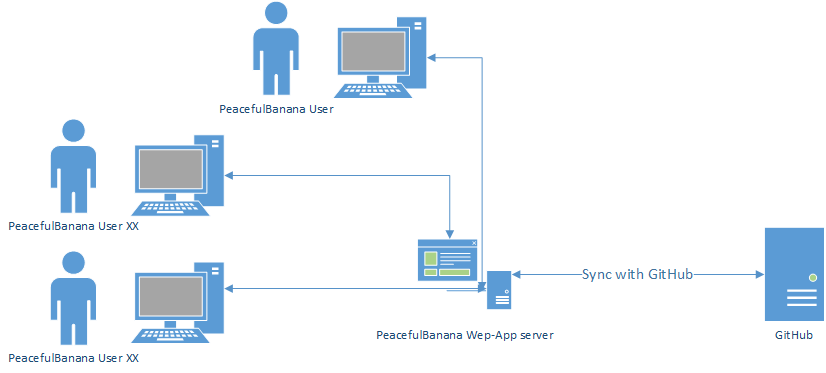
\includegraphics[width=0.8\textwidth]{Clientservergithub}
    \caption{Overview of system design.}
    \label{ClientServerGithub}
\end{figure}

\section{Technology}
% All info om teknologi flyttes hit
When choosing a framework for the prototype, several alternatives like Spring\footnote{\url{http://www.springsource.org/}}, WebObjects\footnote{\url{htpp://www.apple.com/webobjects/}} and Play Framework\footnote{\url{http://www.playframework.com/}} where discussed. Their architecture and our familiarity to the framework was a vital part of the selection. Based on these criteria the server was implemented with Grails a framework for web applications, it is better described in the section following.

\subsubsection{GitHub API}
Skrive litt om github api

\subsection{Grails}
Grails is an open source web application framework which uses the programming language Groovy(which is built on top of the Java Virtual Machine). When Grails was developed, it's developers aimed to re-use proven technologies such as Hibernate, Spring etc. 

\begin{figure}[H]
\centering
    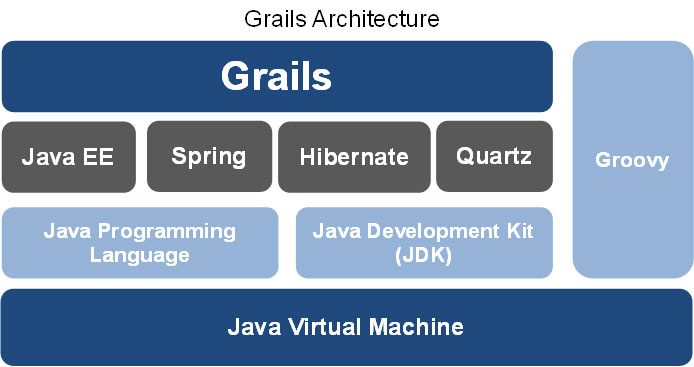
\includegraphics[width=0.8\textwidth]{Grails-Architecture}
\caption{Overview of Grails architecture.}
\end{figure}

Architectural grails is designed with the MVC\footnote{Model View Controller} pattern as a basis, this will expose the model\footnote{Data stored about the object.} in the view\footnote{With the restrictions on what data is viewable for the user.} and any manipulations to the model is done through a controller which controls that the data is correct input to the fields and what fields can be manipulated. An overview of the paradigm can be viewed in figure \ref{mvc-paradigm} below.

This pattern makes it easy for the developer to remain in control when creating a user interface and will ensure that the user can not manipulate fields without going through the controller.

\begin{figure}[H]
    \centering
        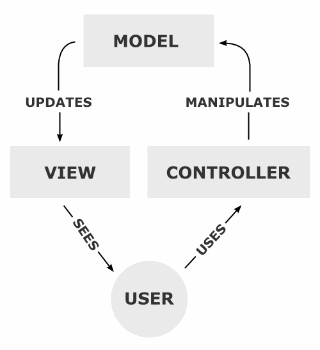
\includegraphics[width=0.5\textwidth]{MVC}
    \caption{Model-view-controller paradigm}
    \label{mvc-paradigm}
\end{figure}

\subsubsection{Server and Database}
% Skriv litt om server og database teknologi her. 

\section{Application Functionality}
% Think it would be wise to show with screenshots the different functionality (the tabs f.ex)
Reflection directed functionality:
\begin{itemize}
\item Collecting data - How a user can retrieve data and annotate it. 
\item Sharing data - How users can work together in groups to collaborate with data. 
\item Reflection triggers - Functionality developed specifically for helping users reflect on their work.
\end{itemize}

\paragraph{Scaffold collected data}\mbox{}\\
Scaffolding is the act of creating a skeleton or a frame for the work to be done. I
PeacefulBanana provides users with the ability to create reflection notes, where they reflect on that day's work and store it for later use. In this context the scaffolding is creating a frame for the reflection to be done, which includes text input and guiding questions. An example of such a reflection note can be seen in Figure \ref{dailynote}. \\
In order to encourage users to reflect on their daily work and to avoid generic or non-constructive input, we connected questions to each input field, to act as guidance. For each input, the application provides a question, like \emph{How did you feel about todays work?} for the mood input. Adding these questions helps users think back on their experiences that day and perform a reflection on these. 
\begin{figure}[H]
    \centering
        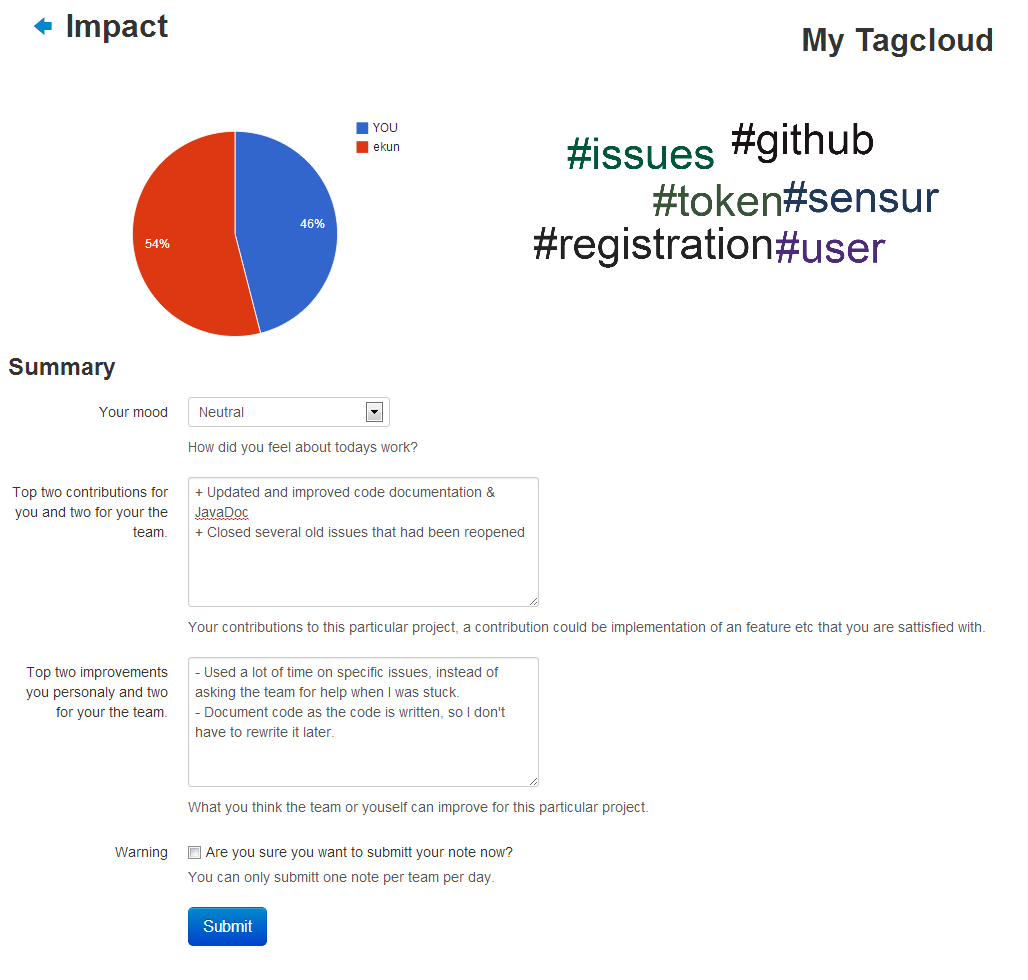
\includegraphics[width=\textwidth]{dailynote}
    \caption{PeacefulBanana reflection note}
    \label{dailynote}
\end{figure}

\paragraph{Tag-clouds}\mbox{}\\
PeacefulBanana also provides the user with individual and team-wide tag-clouds. These tag-clouds are based on the user's or the team's activity in a GitHub project over a period of time. The tag-cloud elements are weighted according to how much the particular \emph{\#tag} has been worked with, the more activity the bigger the word. Implementation of the tag-clouds allows user's to see trending events in their own activity trajectory, but also compare it with the rest of the team. This enables the user to see how their work is affecting the team's work, but also gives the team an indication on what has been worked with over different periods of time(i.e. a development iteration). 
\begin{figure}[H]
    \centering
        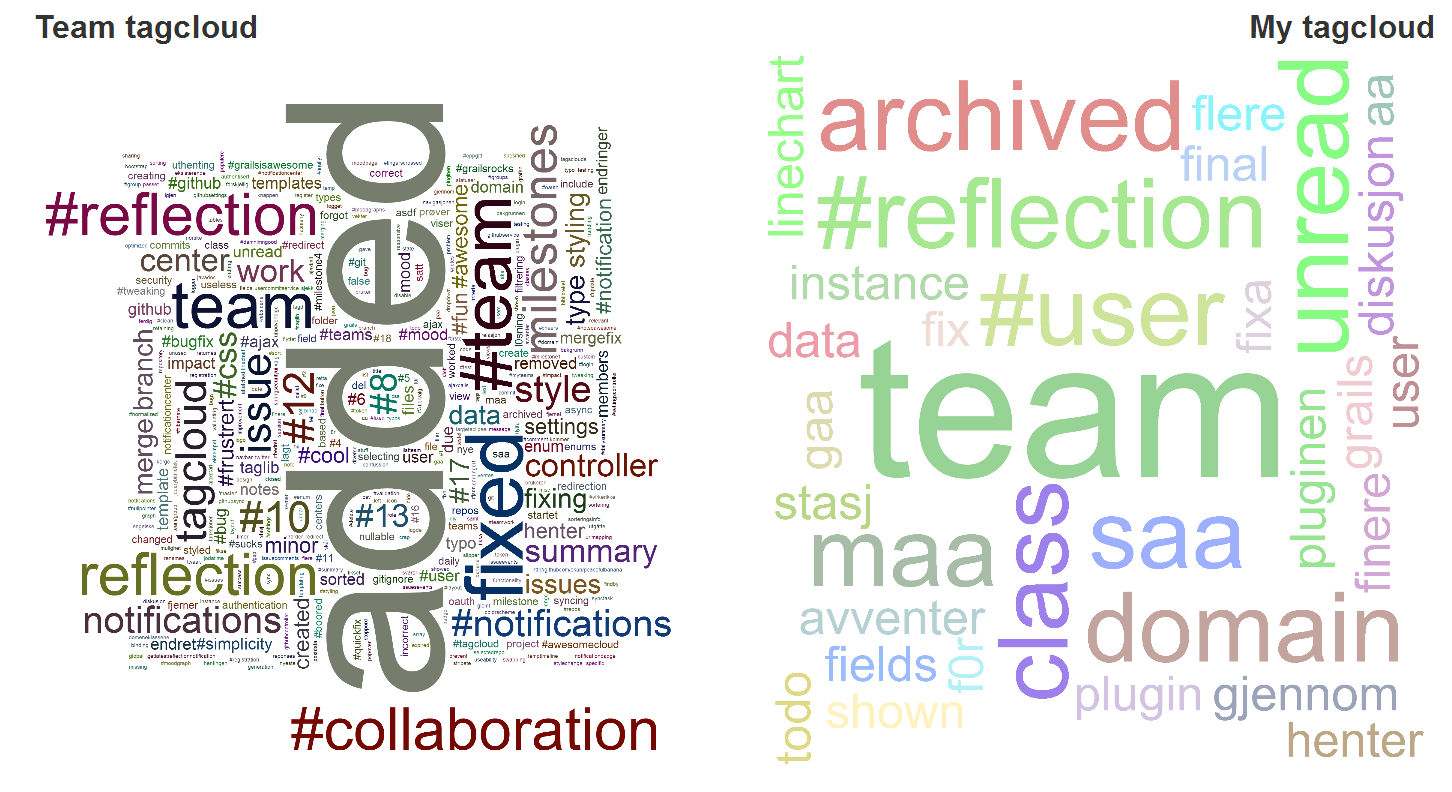
\includegraphics[width=\textwidth]{tagcloud_teamvsmy}
    \caption{PeacefulBanana tag-cloud implementation}
    \label{tagcloudfunc}
\end{figure}

\paragraph{Sharing of data}\mbox{}\\
Reflection notes can be shared with a user's team, should they want to.  PeacefulBanana collects team-relevant data from GitHub , scaffolds and presents these to users. This data gives the team the ability to see who is working on what, are there any trending issues in the team that can be intercepted and solved and more.  
Figure \ref{MyNotes} shows how PeacefulBanana user's can see their notes and the notes' creation date, owning user, what team that user is on and the share status of the note. The user can also simply filter between their own notes or shared notes by their current team. This is shown in Figure \ref{notes_shared}
\begin{figure}[H]
    \centering
        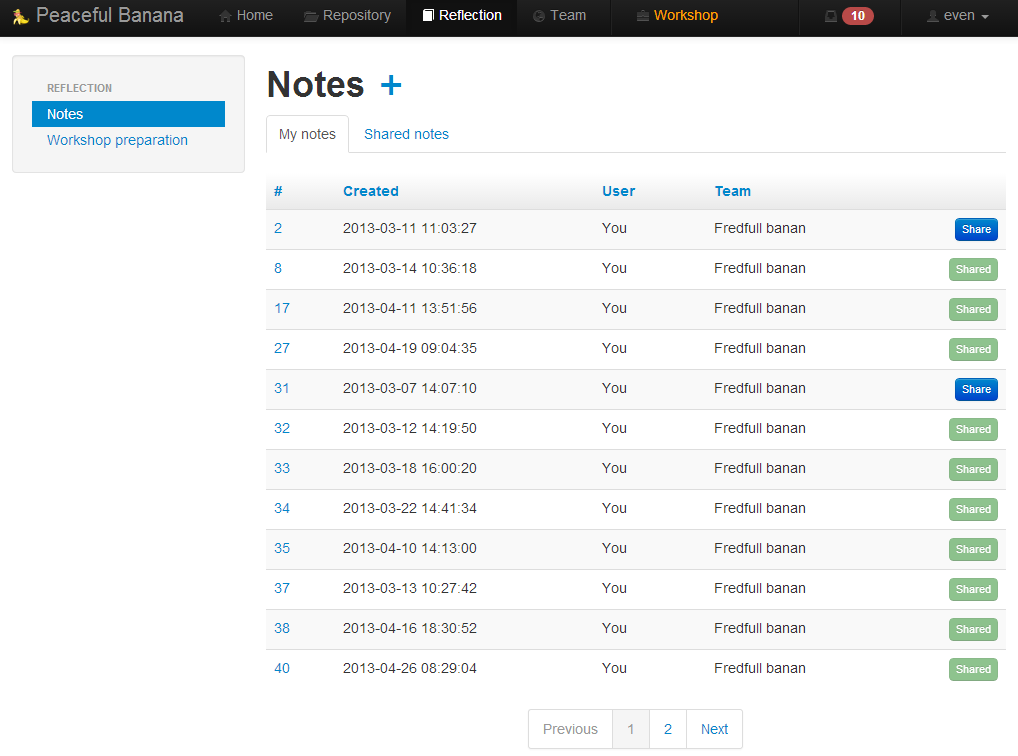
\includegraphics[width=\textwidth]{MyNotes}
    \caption{PeacefulBanana user notes}
    \label{MyNotesFunc}
\end{figure}
\begin{figure}[H]
    \centering
        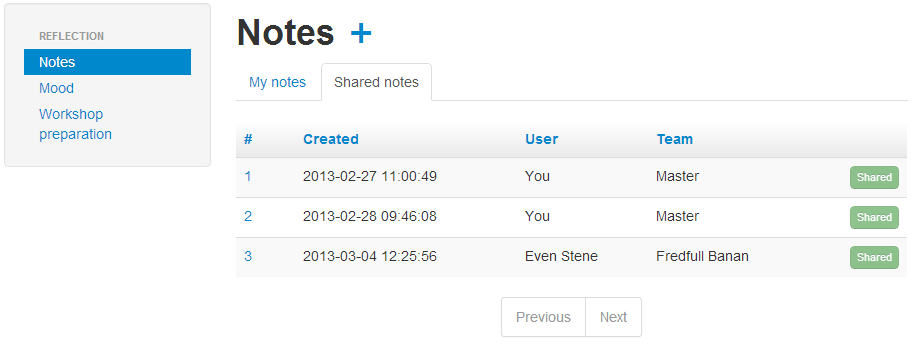
\includegraphics[width=\textwidth]{notes_shared}
    \caption{PeacefulBanana shared team notes}
    \label{notes_sharedfunc}
\end{figure}

\paragraph{Mood graphs}\mbox{}\\
A user can connect his mood to reflection notes. The tool retrieves this mood data daily, in order for the tool to present meaningful mood-averages back to the users. 
The tool allows for presenting this shared team-average mood, giving an indication of how the work is perceived by the other group members and create a discussion around certain trends in mood, or even why certain users stand out from the rest of the team's mood. 

\subsubsection{Milestone example}
% Vise et eksempel fra milestone
\subsubsection{Reflection sessions}
% Vise workshop og hvordan det er tenkt brukt


% Muligens flytte noe av dette til appendix:
\section{Database}
While developing the tool the database was run as a H2\footnote{\url{http://www.h2database.com/}} in-memory database, however the storage was not persistent so we later changed to a MySQL database for the data to stay unchanged when we had to update the tool. This was essential for the tool to function as described in the requirements, but the H2 database was more convenient during development.

In this section we will show how the database is designed as the figure \ref{databaseDomainDiagram} below shows the relationship between the different data types. The data types have been categorized regarding to their origin and are discussed later together with all the fields in each data type.

% Bør denne legge på høykant i appendix?
\begin{figure}[H]
\centering
	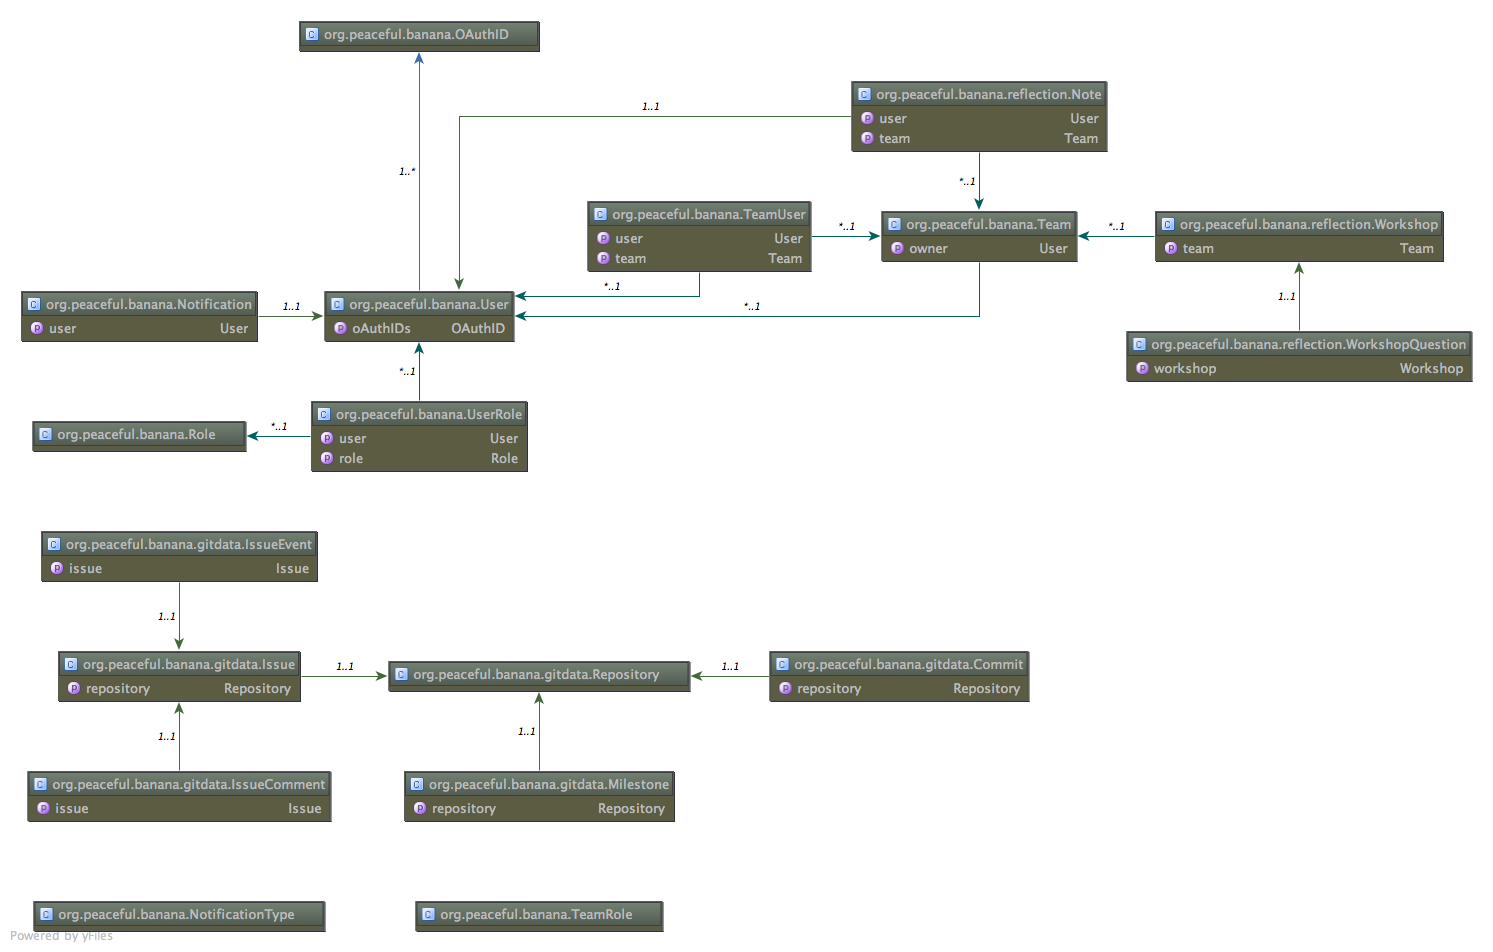
\includegraphics[width=\textwidth]{databaseDomainDiagram}
\caption{Domain diagram, shows the relationship between different classes.}
\label{databaseDomainDiagram}
\end{figure}

\subsection{User data}
The first section is devoted to show and tell all data related to users, the tables below is representing the different data types associated with users. Users are a vital part of the implementation and everything is centered around these users, it is therefore important to store as much relevant data as possible. \\

\subsubsection*{User}
This table hold data related to each user and only the data which is unique to them.
The password are encrypted with SHA-512 encryption which is a part of SHA-2 a set of encryption hashing functions created by the U.S. National Security Agency in 2002 and is a known not to be reversal.\\

\vspace{0.5cm}
\begin{tabularx}{\linewidth}{| c | X |}
    \hline
    \rowcolor[gray]{0.8}
    \textbf{Field} & \textbf{Description} \\
    \hline
    Id & Unique id generated when the user is first created\\ \hline
    UserName & This field stores the users username\\ \hline
   	Password & This field stores the users password as a encrypted string, the password is encrypted with SHA-512 encryption\\ \hline
    Email & This field stores the users email\\ \hline
    FirstName & This field stores the users first name\\ \hline
    LastName & This field stores the users last name\\ \hline
    SelectedRepo & The GitHub generated id of the repository currently selected by the user\\ \hline
    GitLogin & The users GitHub login, used to bind commits to the user\\ \hline
    DateCreated & This field stores the date when the user was first created\\
    \hline
\end{tabularx}
\vspace{0.5cm}

\subsubsection*{Role}
The different roles that the users can be assigned to. These are hierarchy so that the highest gains access to the subset of this access level. \\

\vspace{0.5cm}
\begin{tabularx}{\linewidth}{| c | X |}
    \hline
    \rowcolor[gray]{0.8}
    \textbf{Field} & \textbf{Description} \\
    \hline
    Id & Unique id generated when the role is first created.\\ \hline
    Authority & This field contains the level of authority.\\
    \hline
\end{tabularx}
\vspace{0.5cm}

\subsubsection*{UserRole}
Both fields in this table are combined for the primary key such that each role can only be given to each user once and each users can attain several roles. \\

\vspace{0.5cm}
\begin{tabularx}{\linewidth}{| c | X |}
    \hline
    \rowcolor[gray]{0.8}
    \textbf{Field} & \textbf{Description} \\
    \hline
    User & Foreign key for the users id \\ \hline
    Role & Foreign key for the role id \\
    \hline
\end{tabularx}
\vspace{0.5cm}

\subsubsection*{Notification}
Notifications are used to prompt users about reflection sessions and such. \\

\vspace{0.5cm}
\begin{tabularx}{\linewidth}{| c | X |}
    \hline
    \rowcolor[gray]{0.8}
    \textbf{Field} & \textbf{Description} \\
    \hline
    Id & Unique id generated when the notification is first created\\ \hline
    Title & This field stores the title\\ \hline
   	Body & This field stores the entire message.\\ \hline
    DateCreated & Time stamp generated when the notification is first created.\\ \hline
    Unread & Boolean variable to state if the message is read.\\ \hline
    Cleared & Boolean variable to state if the message is cleared or not.\\ \hline
    NotificationType & The notification type, possible types are 'Reflection' or 'Other'.\\ \hline
    User & A foreign key to the user that received the notification.\\ 
    \hline
\end{tabularx}
\vspace{0.5cm}

\subsection{GitHub data}
In this section we discuss the storage of data collected from GitHub. When we started development we tested with the data stored at GitHub, so we asked GitHub for the data every time it was needed, this made the application slow so we decided to store GitHub data locally to enhance performance. 

When retrieving data from GitHub we used the provided API as described by their developer-site\footnote{\url{http://developer.github.com/v3/}}, this enabled us to control the sequence of data and when to ask for what type of data. All communication to GitHub servers are asynchronous and while therefore not introduce any performance related issues. 

The following data-types where stored in tables as described below.

\subsubsection*{Milestones}
Milestones are major goals consisting of several minor goals called issue, with or without a due date. \\

\vspace{0.5cm}
\begin{tabularx}{\linewidth}{| c | X |}
    \hline
    \rowcolor[gray]{0.8}
    \textbf{Field} & \textbf{Description} \\
    \hline
    GithubId & Unique id from github.com\\ \hline
    Name & The milestones name.\\ \hline
   	Description & A description of the milestone, like what features is to be implemented.\\ \hline
    Status & A variable to say if its open or closed.\\ \hline
    CreatedDate & The time stamp which the milestone is created.\\ \hline
    DueDate & A date which the milestone is due on. This is null if the milestone does not got a due date.\\ \hline
    ClosedDate & A time stamp when the milestone is closed.\\ 
    \hline
\end{tabularx}
\vspace{0.5cm}

\subsubsection*{Issues}
Issues are minor goals or bugs, these issues can be bound to a milestone or independent. \\

\vspace{0.5cm}
\begin{tabularx}{\linewidth}{| c | X |}
    \hline
    \rowcolor[gray]{0.8}
    \textbf{Field} & \textbf{Description} \\
    \hline
    GithubId & Unique id from github.com\\ \hline
    Name & The issues name.\\ \hline
   	Body & A description of the milestone, like what features is to be implemented.\\ \hline
    State & A variable to say if its open or closed.\\ \hline
    Number & A number unique to the repository which is used for referring the issue in the commit messages.\\ \hline
    Repository & A foreign key to the repository it is bound to.\\ \hline
    MilestoneNumber & The milestone which the issue is bound to.\\ \hline
    CreatedAt & The time stamp which the milestone is created.\\ \hline
    UpdatedAt & The time stamp which the milestone last was updated.\\ 
    \hline
\end{tabularx}
\vspace{0.5cm}

\subsubsection*{Commits}
At any given time a developer changes something in the source code it can be committed to the version control system, in this case git/github. These are the commits we store and use for reflection. \\

\vspace{0.5cm}
\begin{tabularx}{\linewidth}{| c | X |}
    \hline
    \rowcolor[gray]{0.8}
    \textbf{Field} & \textbf{Description} \\
    \hline
    GithubId & Unique id from github.com\\ \hline
    Message & The commit message which we gather tags from, these tags are marked hash tags.\\ \hline
   	Login & The GitHub user which did the commit.\\ \hline
    CreatedDate & The time stamp which the commit is created.\\ \hline
    Additions & A date which the milestone is due on. This is null if the milestone does not got a due date.\\ \hline
    Deletions & A time stamp when the milestone is closed.\\ \hline
    Total & A total of lines in the commit.\\
    \hline
\end{tabularx}
\vspace{0.5cm}

\subsubsection*{Repository}
The current data is stored about each repository, in the corresponding fields in the table bellow. \\

\vspace{0.5cm}
\begin{tabularx}{\linewidth}{| c | X |}
    \hline
    \rowcolor[gray]{0.8}
    \textbf{Field} & \textbf{Description} \\
    \hline
    GithubId & Unique id from github.com\\ \hline
    Name & The repository name.\\ \hline
   	Description & A description of the repository.\\ \hline
    CreatedAt & The time stamp which the commit is created.\\ \hline
    UpdatedAt & The time stamp recorded when the milestone last was updated.\\ 
    \hline
\end{tabularx}
\vspace{0.5cm}

\subsection{Collaboration data}
Teams are bound uniquely to a repository, each repository will only have one team bound to it and every user with access\footnote{Being a collaborator of the project on GitHub.} to the repository on GitHub will have the possibility to join the team.  


\subsubsection*{Team}
These teams of users are bound uniquely to a repository and there can only exists one team per repository. \\

\vspace{0.5cm}
\begin{tabularx}{\linewidth}{| c | X |}
    \hline
    \rowcolor[gray]{0.8}
    \textbf{Field} & \textbf{Description} \\
    \hline
    Id & Unique id generated when the team is created.\\ \hline
   	Owner & A foreign key to the user that created the team.\\ \hline
   	Name & The teams name.\\ \hline
    Repository & The githubId of the repository bound to the team.\\ 
    \hline
\end{tabularx}
\vspace{0.5cm}

\subsubsection*{TeamUser}
This contains the users attached to each team and data relevant. \\

\vspace{0.5cm}
\begin{tabularx}{\linewidth}{| c | X |}
    \hline
    \rowcolor[gray]{0.8}
    \textbf{Field} & \textbf{Description} \\
    \hline
    UserId & A foreign key to the users id.\\ \hline
   	TeamId & A foreign key to the teams id.\\ \hline
   	Role & The users role in the team. There are possible roles are 'Manager' and 'Developer'\\ \hline
    Active & A variable that states if the user has selected this team as his active. Only one can be active per user at any given time.\\ 
    \hline
\end{tabularx}
\vspace{0.5cm}

\subsection{Reflection data}
\subsubsection*{Notes}
These notes are bound to a team and there can only be created one for each team by a user each day. \\

\vspace{0.5cm}
\begin{tabularx}{\linewidth}{| c | X |}
    \hline
    \rowcolor[gray]{0.8}
    \textbf{Field} & \textbf{Description} \\
    \hline
    Id & Unique id generated when the note is created.\\ \hline
    Team & A foreign key to the team the note is bound to.\\ \hline
   	User & A foreign key to the user that created the note.\\ \hline
   	Mood & A level regarding the current mood the user that created the note recorded for that day. Mood is recorded as a number between 1-100 where 100 is very happy and 1 is very sad.\\ \hline
   	Contribution & The top 2 contributions done that day for the team by the user.\\ \hline
   	Improvements & The 2 things that can be improved by the user that day for the team.\\ \hline
   	Shared & Variable that states that the note is shared with the team.\\ \hline
    CreatedAt & The time stamp which the commit is created.\\ \hline
    UpdatedAt & The time stamp recorded when the milestone last was updated.\\ 
    \hline
\end{tabularx}
\vspace{0.5cm}

\subsubsection*{Workshop}
Managers or owners of teams can create reflection workshops, where it is generated a set of questions based on the tags used by the teams members in the selected period. \\

\vspace{0.5cm}
\begin{tabularx}{\linewidth}{| c | X |}
    \hline
    \rowcolor[gray]{0.8}
    \textbf{Field} & \textbf{Description} \\
    \hline
    Id & Unique id generated when the workshop is created.\\ \hline
   	TeamId & A foreign key to the team.\\ \hline
   	CreatedAt & The time stamp which the workshop is created.\\ \hline
   	DurationStart & The time stamp which the workshop period starts.\\ \hline
   	DateStart & The time stamp which the workshop period ends.\\ 
    \hline
\end{tabularx}
\vspace{0.5cm}

\subsubsection*{WorkshopQuestions}
This table holds the questions for each workshop and indicates if they are mandatory or not. \\

\vspace{0.5cm}
\begin{tabularx}{\linewidth}{| c | X |}
    \hline
    \rowcolor[gray]{0.8}
    \textbf{Field} & \textbf{Description} \\
    \hline
    Id & Unique id generated when the question is created.\\ \hline
   	Workshop & A foreign key to the workshop.\\ \hline
   	QuestionText & The generated question.\\ \hline
   	CommitTag & The tag which the question is generated from.\\ 
    \hline
\end{tabularx}
\vspace{0.5cm}

\section{User Interface}
When implementing the design as discussed in the earlier chapter, we had a lot of focus on creating a simpler yet informative page-layout and it is because of this we 

When designing the Peaceful Banana, it was clear that our task required a lot of design work. In order to create a simple yet informative page-layout the twitter bootstrap framework was chosen.

The design itself is heavily based on the fluid layout and sign in examples from the official examples.

\subsection{Twitter bootstrap}
Twitter bootstrap is a front-end framework for easier and faster web development, it is widely used and makes it possible to create beautiful web pages without much work. Bootstrap utilizes both HTML5 and CSS3 standards.

\subsection{jQuery}
It was initially released under the MIT license in 2006 to make it easier to select DOM\footnote{Document-Object-Model} objects and create powerful dynamic web pages and applications.

JQuery has been used for AJAX\footnote{Asynchronous JavaScript and XML}, this is a way to change the contents DOM objects asynchronous from JavaScript.

\subsubsection{AwesomeCloud}
Awesome cloud is a plugin for jQuery for creating a tag cloud, it retrieves data from DOM-objects and rendered them as a cloud where the font-size increases with the occurrence of tags, the tag cloud is then drawn on the HTML5 canvas.
